\subsection{Fused Pipeline}
\label{sec:results_fused}

\subsubsection{Konzept}
In der bisher betrachteten Konfiguration wird nach jeder Pipeline-Stufe
das Zwischenergebnis vom Device zurück auf den Host kopiert und im
nachfolgenden Schritt erneut auf das Device übertragen, obwohl die
Daten dort direkt weiterverarbeitet werden könnten. Die Fused Pipeline
(aktivierbar über \texttt{FUSED\_PIPELINE=1}, siehe
Abschnitt~\ref{subsec:build-system-und-kompilierung}) verzichtet auf diese
redundanten H$\to$D/D$\to$H-Transfers zwischen den vier Stufen: Das
Eingabebild wird einmalig auf das Device kopiert, alle vier Kernel
(Gaussian Blur, Sobel, Non-Maximum Suppression, Hysteresis) laufen
anschließend nacheinander auf denselben Device-Buffern, und lediglich
das finale Ergebnis wird am Ende einmalig zurück auf den Host kopiert.

\subsubsection{Performance}
Abbildung ~\ref{fig:fused_comparison_combined} vergleicht die Summe der isoliert gemessenen
Einzelschritte (jeweils mit eigenem H$\to$D/D$\to$H-Transfer) mit der
Fused Pipeline, die nur einmalig zu Beginn und am Ende transferiert.

\begin{figure}[H]
    \centering
    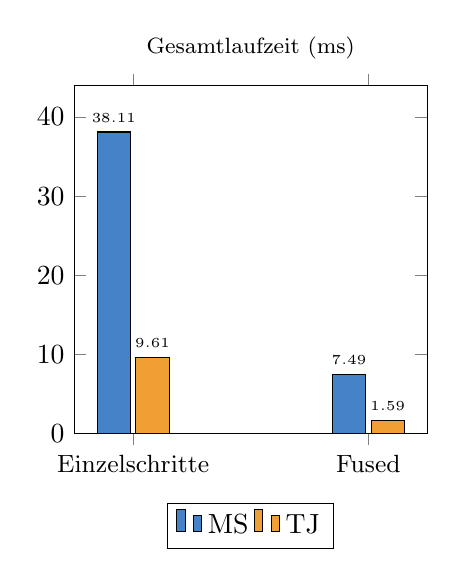
\begin{tikzpicture}
        \begin{axis}[
            ybar,
            bar width=12pt,
            title={Gesamtlaufzeit (ms)},
            title style={font=\footnotesize},
            symbolic x coords={Einzelschritte, Fused},
            xtick=data,
            xticklabel style={font=\small},
            width=0.5\textwidth,
            height=6cm,
            ymin=0, ymax=44,
            enlarge x limits=0.25,
            nodes near coords,
            nodes near coords style={font=\tiny},
            legend style={at={(0.5,-0.2)}, anchor=north, legend columns=2},
        ]
            % MS-Messung
            \addplot[fill={rgb,255:red,70;green,130;blue,200}]
                coordinates {(Einzelschritte,38.108) (Fused,7.494)};
            % TJ-Messung
            \addplot[fill={rgb,255:red,240;green,160;blue,50}]
                coordinates {(Einzelschritte,9.613) (Fused,1.590)};
            
            \legend{MS, TJ}
        \end{axis}
    \end{tikzpicture}
    \caption{Fused Pipeline vs. Summe der isolierten Einzelschritte für MS- und TJ-Messungen.}
    \label{fig:fused_comparison_combined}
\end{figure}


Durch den Wegfall der redundanten Zwischentransfers sinkt die Gesamtlaufzeit
um 30.615\,ms bzw. 80.3\,\%. Da jede Stufe zuvor ihr Ergebnis erst auf den
Host und im nächsten Schritt wieder auf das Device kopierte, macht dieser
Overhead den Großteil der isolierten Gesamtzeit aus, während die eigentliche
Kernel-Rechenzeit vergleichsweise gering bleibt. Ein ähnliches Verhältnis zeichnet sich auch bei Thomas Jurczyk ab (siehe Abbildung ~\ref{fig:fused_comparison_combined}), bei dessen Messungen sich die Laufzeit von 9.613 ms auf 1.590 ms verbessert, was einem Speedup von etwa 6 entspricht.
